\documentclass[12pt]{report}
\usepackage{subfigure}
\usepackage[utf8]{vietnam}
\usepackage[left=2.50cm, right=2.00cm, top=2.00cm, bottom=2.00cm]{geometry}
\usepackage{fancybox,graphicx}
\usepackage{mathrsfs} 
\usepackage{amsfonts}
\usepackage{longtable,array}
\usepackage{multirow}
\newlength\mylength
\newcolumntype{C}[1]{>{\centering\arraybackslash}p{#1}}
\usepackage[intlimits]{amsmath}
\usepackage{array}
\usepackage[unicode]{hyperref}
\usepackage{adjustbox}
% \usepackage{algorithm}
% \usepackage{algorithmicx}
\makeatletter
% \renewcommand{\ALG@name}{Thuật toán}
\makeatother
\usepackage{algpseudocode}
\usepackage{caption}
\usepackage{amsxtra,amssymb,latexsym,amscd,amsthm}
\usepackage{enumitem}
\usepackage{tikz}
\usepackage{makeidx}
\usepackage{float}
\usepackage{xcolor}
% \usetikzlibrary{shapes.geometric}
% \usetikzlibrary{positioning,automata}
% \usepackage{scrextend}
% \usepackage{longfbox}
%Môi trường Lời giải
%\newtheorem{theorem}{Định lý}[chapter]
%\newtheorem{definition}{Định nghĩa}[chapter]
%\newtheorem{example}{Ví dụ}[chapter]
%\newtheorem{lemma}[theorem]{Bổ đề}
%Tiêu đề
% \newtheorem{pro}{Bài toán}
% \newtheorem*{constr}{Ràng buộc}
% \newtheorem*{calfunc}{Các hàm được thực thi}
% \newtheorem*{Sol}{Giải thuật}
% \newtheorem*{Anal}{Phân tích giải thuật}

% \usepackage{fancyhdr}
% \pagestyle{fancy}
% \lhead{}
% \chead{}
% \rhead{Nguyên lý Hệ Điều Hành}
% \lfoot{}
% \cfoot{\thepage}
% \rfoot{}

\paperheight=24cm
\paperwidth=17cm
\textwidth=13truecm
\textheight=19,7truecm
\topmargin=0cm
\headsep=20truept
\headheight=12pt
\voffset=-0.75truecm
\hoffset=-0.75cm
\oddsidemargin=0.5cm
\evensidemargin=0.5cm
\footskip=30 pt
\pagenumbering {arabic}
\setcounter{page}{1}
\setcounter{chapter}{0}
\addtocontents{toc}{\protect\vspace{20pt}}

\usepackage{xcolor}
\usepackage{listings}
\usepackage{titlesec}
\usepackage[bottom]{footmisc}

\titleformat{\chapter}[display]
{\normalfont\huge\bfseries}{\chaptertitlename\ \thechapter}{20pt}{\Huge}
\titlespacing*{\chapter}{0pt}{-50pt}{40pt}

% \renewcommand{\thechapter}{\Roman{chapter}}
% \renewcommand{\thesection}{\thechapter.\Roman{section}}
% \renewcommand{\thesubsection}{\thesection.\Roman{subsection}}

\definecolor{mGreen}{rgb}{0,0.6,0}
\definecolor{mGray}{rgb}{0.5,0.5,0.5}
\definecolor{mPurple}{rgb}{0.58,0,0.82}
\definecolor{backgroundColour}{rgb}{0.95,0.95,0.92}
\setcounter{secnumdepth}{4}
\setcounter{tocdepth}{4}

\lstdefinestyle{CStyle}{
	backgroundcolor=\color{backgroundColour},
	commentstyle=\color{mGreen},
	keywordstyle=\color{magenta},
	numberstyle=\tiny\color{mGray},
	stringstyle=\color{mPurple},
	basicstyle=\footnotesize,
	breakatwhitespace=false,
	breaklines=true,
	captionpos=b,
	keepspaces=true,
	numbers=left,
	numbersep=5pt,
	showspaces=false,
	showstringspaces=false,
	showtabs=false,
	tabsize=2,
	language=C
}


% \renewcommand{\fboxrule}{0.3pt}

\begin{document}

\thispagestyle{empty}


\begin{titlepage}
	\begin{figure}[h]
		\centering
		
\includegraphics[width=0.5\textwidth]{images/logotmh.png}
	\end{figure}

	\begin{center}
		\textbf{{\Huge CUỘC THI}} \\[10pt]
		\textbf{\LARGE TOÁN MÔ HÌNH 2023}\\[10pt]
		\textbf{\LARGE VÒNG 1}\\[10pt]
		\textbf{ 01 tháng 08  - 20 tháng 08, 2023}
		\\[3.0cm]

		\begin{tabular}{r l}
			\textbf{Tên đội thi}: &APM \\
			\textbf{Thành viên:}
				&$-$ Nguyễn Thành Phát \\
				&$-$ Lê Xuân An \\
				&$-$ Phạm Công Minh
		\end{tabular}
	\end{center}

	\vspace{\fill}
\end{titlepage}

\newpage

\tableofcontents
% \renewcommand{\thechapter}{\arabic{chapter}}
% \renewcommand{\thesection}{\thechapter.\arabic{section}}
% \renewcommand{\thesubsection}{\thesection.\arabic{subsection}}
% \newcounter{chapter}{0}

\chapter*{Thông tin cần thiết về bài toán}
\addcontentsline{toc}{chapter}{Thông tin cần thiết về bài toán}
\section*{Giới thiệu sơ bộ về tỉnh Quảng Bình}
\addcontentsline{toc}{section}{Giới thiệu sơ bộ về tỉnh Quảng Bình}
\begin{flushleft}
	Tỉnh Quảng Bình là một tỉnh nằm ở phía Bắc miền Trung Việt Nam, giáp biên giới với Lào. Tỉnh này có vị trí chiến lược trên tuyến đường biển Bắc - Nam của Việt Nam, và nổi tiếng với các danh lam thắng cảnh độc đáo, cùng với lịch sử và văn hóa đa dạng.
	\\[\baselineskip]

	\begin{figure}[H]
		\centering
		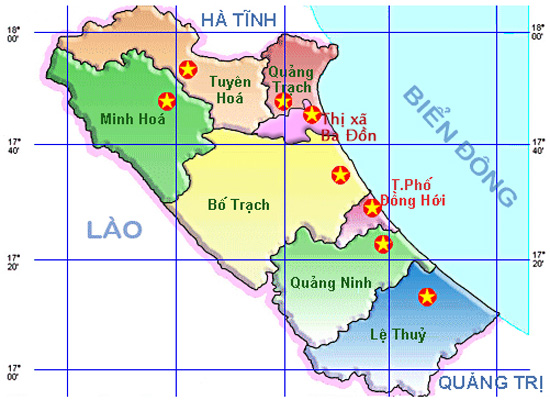
\includegraphics[width = \textwidth]{images/BandoQB.png}
		\caption{Bản đồ hành chính tỉnh Quảng Bình}
	\end{figure}
\end{flushleft}

\newpage

\section*{Đặc điểm khí hậu của tỉnh Quảng Bình} % (fold)
\addcontentsline{toc}{section}{Đặc điểm khí hậu của tỉnh Quảng Bình}
\begin{flushleft}
	Quảng Bình thuộc vùng khí hậu nhiệt đới, chia thành hai mùa rõ rệt là mùa mưa và mùa khô. Dưới đây là mô tả sơ bộ về khí hậu của Quảng Bình:
	\begin{itemize}
		\item \textbf{Mùa mưa (mùa hè)}: Thường kéo dài từ tháng 9 đến tháng 3 năm sau. Trong khoảng thời gian này, tỉnh thường trải qua mưa nhiều và độ ẩm cao. Mùa mưa thường đem lại lượng mưa lớn, có thể gây ra lũ lụt và ngập úng tùy thuộc vào từng năm.

		\item \textbf{Mùa khô (mùa đông)}: Bắt đầu từ tháng 4 đến tháng 8. Trong mùa này, Quảng Bình thường trải qua ít mưa hơn và thời tiết khô ráo hơn. Nhiệt độ thường ổn định hơn so với mùa mưa.
	\end{itemize}

	Trong cả hai mùa, nhiệt độ ở Quảng Bình không có sự biến đổi lớn và thường duy trì ở mức ấm áp. Nhiệt độ trung bình hàng ngày dao động từ 22 đến 27 độ C, tùy thuộc vào mùa và thời điểm trong ngày. Mùa hè có thể có nhiệt độ cao hơn và cảm nhận nóng bức do tác động của ánh nắng mặt trời.
	\\[\baselineskip]

	Các biến đổi khí hậu và thời tiết trong Quảng Bình cũng ảnh hưởng đến việc trồng trọt và sản xuất nông nghiệp. Những biện pháp ứng phó với lũ lụt, ngập úng, và thiếu nước cần được đưa ra để đảm bảo sự ổn định trong sản xuất nông nghiệp và đời sống cộng đồng trong khu vực này.
	\\[\baselineskip]

	Trung bình, mỗi năm tỉnh Quảng Bình đối mặt với 5-6 cơn bão và/hoặc áp thấp nhiệt đới. Tháng VIII, tháng IX và tháng X là những tháng mà bão thường xuyên xảy ra. Lũ dâng cao xảy ra ở các vùng đất và thung lũng thấp của tỉnh khi có 3 yếu tố diễn ra cùng một thời điểm: lượng mưa lớn, dòng chảy lớn từ thượng nguồn và thủy triều cao từ biển. Lũ lớn gây ra nhiều mất mát và thiệt hại cho cộng đồng.
\end{flushleft}

\chapter{Bài toán 1}
\section{Ý (a)} % (fold)

\begin{flushleft}
	Nông nghiệp nói chung và canh tác lúa có quan hệ qua lại và phức tạp đối với nhiều điều kiện, trong đó các yếu tố khí hậu là những nhân tố tác động mãnh mẽ nhất. Những ảnh hưởng của khí hậu, thời tiết đến sản xuất nông nghiệp được thể hiện qua đại lượng năng suất (cao hay thấp) và chất lượng nông sản (tốt hay xấu).
	\\[\baselineskip]

	Những điều kiện khí hậu thời tiết được xác định cho việc canh tác lúa trước hết là ánh sáng, nhiệt độ và nước. Đó là những yếu tố thiết yếu với sự sinh trưởng phát triển và cấu thành năng suất cây trồng và động vật. Chúng ta dễ dàng thấy rằng, để trồng được một cây lúa cần phải đảm bảo một lượng nhiệt (tổng nhiệt độ) nhất định, đồng thời phải có một lượng nước cần thiết trong tầng đất canh tác cho cả một thời kỳ sinh trưởng, phát triển. Bên cạnh đó, biến đổi khí hậu đóng vai trò rất quan trọng trong năng suất của cây lúa.
\end{flushleft}

\subsection{Ảnh hưởng của ánh sáng đến cây lúa} % (fold)
\label{sub:ảnh_hưởng_của_ánh_sáng_đến_cây_lúa}
\begin{flushleft}
	Ánh sáng có mối quan hệ quan trọng với sự phát triển của cây lúa và các loại cây khác. Dưới đây là một số điểm nổi bật về mối quan hệ này:

	\begin{itemize}
		 \item \textbf{Quá trình quang hợp}: Ánh sáng là yếu tố quan trọng nhất trong quá trình quang hợp, nơi cây lúa chuyển đổi ánh sáng mặt trời thành năng lượng thông qua việc sản xuất glucose từ nước và carbon dioxide. Glucose sau đó được dùng làm nhiên liệu cho các hoạt động của cây và giúp cây lúa phát triển.

		 \item \textbf{Chỉnh sửa sinh học}: Ánh sáng ảnh hưởng đến nhiều quá trình sinh học khác nhau trong cây lúa, chẳng hạn như sự mở rộng của lá, sự phát triển của rễ, và sự chín của bông lúa.

		 \item \textbf{Photoperiodism}: Một số giống lúa phản ứng với độ dài của ngày ánh sáng, gọi là photoperiodism. Điều này ảnh hưởng đến thời điểm cây ra hoa và thời gian thu hoạch. Sự hiểu biết về photoperiodism giúp nhà nghiên cứu và nông dân lựa chọn giống lúa phù hợp với điều kiện ánh sáng cụ thể của khu vực họ trồng.

		 \item \textbf{Nhiệt độ}: Ánh sáng mặt trời cũng là nguồn nhiệt độ quan trọng, ảnh hưởng đến sự phát triển và sinh trưởng của cây lúa.

		 \item \textbf{Kích thích sự phát triển}: Ánh sáng có khả năng kích thích sự phát triển của cây lúa thông qua việc ảnh hưởng đến các hoạt động hóa học và sinh lý.

		 \item \textbf{Quản lý sâu bệnh}: Ánh sáng cũng có thể ảnh hưởng đến sự xuất hiện và phát triển của một số loại sâu bệnh, ảnh hưởng đến năng suất và chất lượng của cây lúa.
	\end{itemize}

	Để đạt được năng suất tốt và chất lượng hạt lúa cao, việc quản lý và tối ưu hóa nguồn ánh sáng cho cây lúa là rất quan trọng.
	\\[\baselineskip]

	\begin{figure}[h!]
		\centering
		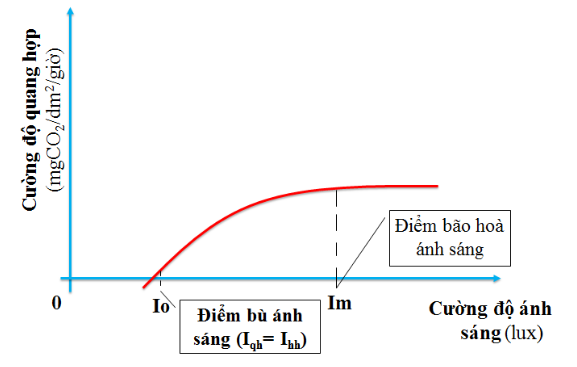
\includegraphics[width = 0.9\textwidth]{images/sodoanhsang.png}
		\caption{Ảnh hưởng của ánh sáng đến với cường độ quang hợp của cây trồng}
	\end{figure}
\end{flushleft}
% subsection ảnh_hưởng_của_ánh_sáng_đến_cây_lúa (end)

\subsection{Ảnh hưởng của nhiệt độ đến cây lúa} % (fold)
\label{sub:ảnh_hưởng_của_nhiệt_độ_đến_cây_lúa}
\begin{flushleft}
	Nhiệt độ là một trong những yếu tố quan trọng ảnh hưởng đến sự sinh trưởng và phát triển của cây lúa. Dưới đây là một số cách mà nhiệt độ có thể ảnh hưởng đến lúa:

	\begin{itemize}
		\item \textbf{Nảy mầm}: Để hạt lúa nảy mầm tốt, nhiệt độ tối ưu thường nằm trong khoảng từ 25°C đến 35°C. Nếu nhiệt độ quá thấp hoặc quá cao, tỉ lệ nảy mầm có thể giảm.

		\item \textbf{Sự sinh trưởng của cây non}: Nhiệt độ quá cao hoặc quá thấp có thể làm giảm tốc độ sinh trưởng của cây non và giảm năng suất.

		\item \textbf{Quá trình hình thành bông}: Nhiệt độ quá cao vào thời điểm hình thành bông có thể làm giảm số lượng hạt trên mỗi bông và giảm chất lượng hạt.

		\item \textbf{Quá trình ra hoa và thụ phấn}: Nhiệt độ quá cao hoặc quá thấp có thể ảnh hưởng đến quá trình ra hoa và thụ phấn, làm giảm năng suất.

		\item \textbf{Chất lượng hạt}: Nhiệt độ ổn định và mát mẻ ở giai đoạn cuối cùng của sự phát triển hạt có thể giúp cải thiện chất lượng hạt.

		\item \textbf{Tốc độ chín}: Nhiệt độ cao có thể tăng tốc độ chín của lúa, nhưng cũng có thể làm giảm chất lượng hạt.

		\item \textbf{Bệnh và sâu hại}: Nhiệt độ cũng ảnh hưởng đến sự phát triển và sinh sản của nhiều loại bệnh và sâu hại.

		\item \textbf{Tích trữ nước}: Nhiệt độ cao làm gia tăng sự bay hơi nước từ mặt đất và từ lá cây, dẫn đến nhu cầu nước tăng lên.
	\end{itemize}

	Nói chung, việc quản lý và kiểm soát nhiệt độ trong quá trình trồng lúa rất quan trọng để đạt được năng suất và chất lượng tốt.
	\\[\baselineskip]

	\begin{figure}[H]
		\centering
		\caption{Liên hệ giữa nhiệt độ và năng suất lúa}
		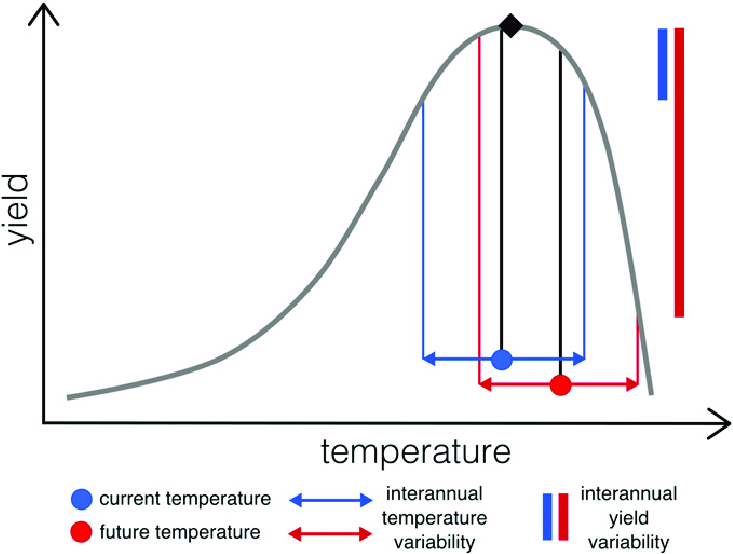
\includegraphics[width = \textwidth]{images/sodonhietdo.png}
	\end{figure}

	Biểu đồ mô tả quan hệ giữa nhiệt độ và năng suất. Trong trường hợp không lai tạo để chịu nhiệt, việc tăng nhiệt độ trung bình vượt quá nhiệt độ tối ưu (${\blacklozenge}$) sẽ dẫn đến giảm năng suất trung bình và tăng biến động của năng suất, giả sử biến động nhiệt độ hàng năm vẫn không đổi.
\end{flushleft}
% subsection ảnh_hưởng_của_nhiệt_độ_đến_cây_lúa (end)

\subsection{Ảnh hưởng của lượng nước đến cây lúa} % (fold)
\label{sub:ảnh_hưởng_của_lượng_nước_đến_cây_lúa}
\begin{flushleft}
	\textbf{Nhu cầu nước của lúa}: Nói chung nhu cầu nước của cây lúa lớn hơn so với một số cây trồng khác. Trước đây, ở nước ta cũng như một số nước trong khu vực, khi chưa có công trình thủy lợi thì hàng năm chỉ gieo cấy được một vụ vào mùa mưa. Nguồn nước mưa rất quan trọn, nó không chỉ cung cấp nước cho cây trồng sinh trưởng và phát triển mà còn làm thay đổi tiểu khí hậu trong ruộng lúa. Những cơn mưa nhiệt đới mang đến nguồn đạm từ khí trời và mang đến nguồn ôxi cho ruộng lúa. Trong điều kiện thủy lợi chưa hoàn chỉnh, hoặc hệ thống công trình xuống cấp hoặc hồ chứa không xả nước thì lượng mưa là một trong những yếu tố quyết định đến việc hình thành các vùng trồng lúa và các vụ lúa trong năm. Trong mùa mưa ẩm, lượng mưa cần thiết cho cây lúa trung bình là 6-7mm/ngày và 8-9mm/ngày trong mùa khô nếu không có các nguồn nước khác bổ sung. Nếu tính luôn lượng nước thấm và bốc hơi thì trung bình một tháng cây lúa cần khoảng 200mm nước mưa và trong cả vụ lúa cần 1000mm, chưa kể lượng nước cần thiết để gieo mạ.

	\begin{figure}[!htbp]
		\centering
		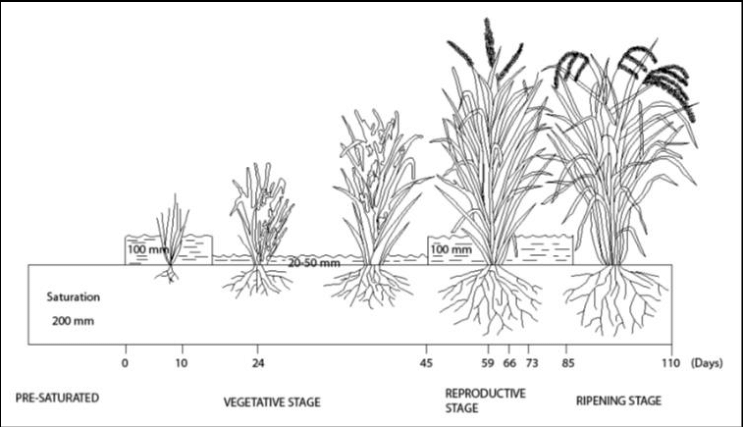
\includegraphics[width = \textwidth]{images/sodonuoc.png}
		\caption{Biểu đồ nước cho cây lúa}
	\end{figure}
\end{flushleft}
% subsection ảnh_hưởng_của_lượng_nước_đến_cây_lúa (end)

\subsection{Ảnh hưởng của biến đổi khí hậu đến với năng suất lúa} % (fold)
\label{sub:ảnh_hưởng_của_biến_đổi_khí_hậu_đến_với_năng_suất_lúa}
\begin{flushleft}
	Biến đổi khí hậu đang và sẽ tiếp tục tác động mạnh mẽ đến năng suất lúa vì yếu tố này sẽ ảnh hưởng trực tiếp đến nhiệt độ, lượng nước mưa và chất lượng không khí.

	\begin{itemize}
		\item \textbf{Tăng nhiệt độ}: Lúa, đặc biệt là lúa nước, yêu cầu một nhiệt độ ổn định trong quá trình sinh trưởng. Tăng nhiệt độ có thể gây ảnh hưởng đến quá trình hình thành bông và làm giảm năng suất hạt. Nhiệt độ đêm tăng cao có thể giảm năng suất lúa do giảm sự tích luỹ chất dinh dưỡng trong quá trình photosynthesis.

		\item \textbf{Thay đổi mức lượng mưa}: Một số khu vực có thể trải qua giai đoạn hạn hán kéo dài, trong khi khu vực khác lại chịu cảnh lũ lụt thường xuyên hơn. Cả hai tình huống này đều ảnh hưởng tiêu cực đến năng suất lúa. Sự biến động không lường trước về mưa có thể gây ra khó khăn trong việc lên kế hoạch trồng trọt, đặc biệt là trong những khu vực phụ thuộc vào mùa mưa.

		\item \textbf{Tăng nồng độ $CO_2$}: Việc tăng nồng độ $CO_2$ có thể tăng cường quá trình quang hợp, giúp cây lúa phát triển nhanh hơn. Tuy nhiên, lợi ích này có thể bị giảm sút nếu không có đủ nước và dinh dưỡng. Các nghiên cứu đã chỉ ra rằng, dù $CO_2$ giúp tăng năng suất, nhưng chất lượng hạt lúa (như hàm lượng protein) có thể bị giảm.

		\item \textbf{Sự gia tăng của các sự kiện khí hậu cực đoan}: Sự gia tăng về số lần và mức độ của các sự kiện khí hậu cực đoan như bão, hạn hán và lũ lụt có thể gây ra tổn thất lớn cho vụ mùa.

		\item \textbf{Ảnh hưởng đến dịch hại và bệnh tật}: Biến đổi khí hậu có thể tạo điều kiện thuận lợi cho sự phát triển và lan rộng của các loại dịch hại và bệnh tật trên cây lúa, làm giảm năng suất và chất lượng sản phẩm.

		\item \textbf{Thay đổi về môi trường sinh thái}: Biến đổi khí hậu có thể làm thay đổi môi trường sinh thái xung quanh, ảnh hưởng đến độ mặn của nước trong khu vực trồng lúa ven biển hay thay đổi mức nước ngầm ở một số khu vực.
	\end{itemize}

	Những tác động trên đều yêu cầu các nhà nghiên cứu, nhà quản lý và người nông dân phải tìm kiếm giải pháp để thích nghi và giảm thiểu hậu quả của biến đổi khí hậu đối với ngành sản xuất lúa.
\end{flushleft}
% subsection ảnh_hưởng_của_biến_đổi_khí_hậu_đến_với_năng_suất_lúa (end)

\newpage

\section{Ý (b)} % (fold)

\begin{flushleft}
	Sau khi đã tìm hiểu từ các nguồn, đội đã tổng hợp được sản lượng lúa của Quảng Bình từ năm 2000 - 2022
	\\[\baselineskip]

	\begin{figure}[!htbp]
		\centering
		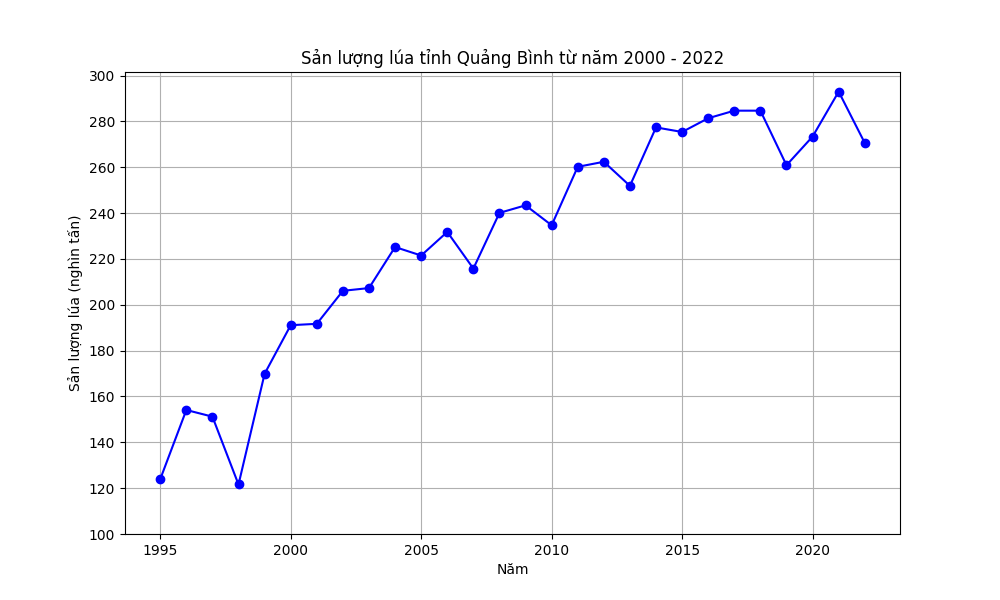
\includegraphics[width = \textwidth]{images/sanluonglua.png}
		\caption{Sản lượng lúa của Quảng Bình từ năm 2000 - 2022}
	\end{figure}
\end{flushleft}
% section ý_ (end)

\newpage

\section{Ý (c)} % (fold)

\begin{flushleft}
	Sau khi đã tìm hiểu từ các nguồn, đội đã tổng hợp được các cơn bão đổ bộ vào khu vực miền Trung nói chung và Quảng Bình nói riêng trong giai đoạn 2000 - 2022.
	\\[\baselineskip]

	\begin{table}[!ht]
		% \centering
		\captionsetup{justification = centering}
		\caption{Các cơn bão đổ bộ vào khu vực miền Trung và Quảng Bình giai đoạn 2000 - 2022}
		\begin{adjustbox}{width = 1.2\linewidth, center}
		\begin{tabular}{|l|l|l|l|l|l|}
		\hline
			Thứ tự & Bão & Thời gian đổ bộ & Thời gian kết thúc & Cấp độ lúc đổ bộ & Đổ bộ \\ \hline
			1 & Wutip & 30/9/2013 & 1/10/2013 & 12 & Quảng Bình \\ \hline
			2 & Doksuri & 15/9/2017 & 16/9/2017 & 12, 13 & Quảng Bình \\ \hline
			3 & Sinlaku & 2/8/2020 & 5/8/2020 & 7 & Thanh Hóa \\ \hline
			4 & Noul & 18/9/2020 & 19/9/2020 & 8, 9 & Huế \\ \hline
			5 & Saudel & 26/10/2020 & 26/10/2020 & 6, 7 & Đã suy yếu thành ÁTNĐ\footnotemark[1] khi đổ bộ vào Quảng Bình \\ \hline
			6 & Molave & 28/10/2020 & 29/10/2020 & 13 & Quảng Ngãi \\ \hline
			7 & Vamco & 15/11/2020 & 17/11/2020 & 8.5 & Quảng Bình \\ \hline
			8 & Podul & 30/08/2019 & 31/9/2019 & 9 & Quảng Bình \\ \hline
			9 & Damrey & 4/11/2017 & 5/11/2017 & 12 & Khánh Hòa \\ \hline
			10 & Lekima & 3/10/2007 & 4/10/2007 & 12 & Quảng Bình \\ \hline
			11 & Bão số 5 (ÁTNĐ\footnotemark[1] 17W) & 23/9/2006 & 25/9/2006 & 8 & Quảng Bình \\ \hline
			12 & Sơn Tinh & 18/7/2018 & 22/7/2018 & 6.5 & Suy yếu thành ÁTNĐ\footnotemark[1] \\ \hline
			13 & Talas & 17/7/2017 & 17/7/2017 & 10 & Hà Tĩnh \\ \hline
			14 & Ketsana & 26/9/2009 & 30/9/2009 & 13 & Quảng Ngãi \\ \hline
			15 & Xangsane & 1/10/2006 & 2/10/2006 & 13 & Đà Nẵng \\ \hline
			16 & Usagi & 10/8/2001 & 11/8/2001 & 8 & Quảng Bình \\ \hline
			17 & Mekkhala & 28/9/2008 & 30/9/2008 & 9 & Quảng Bình \\ \hline
			18 & Wukong & 9/9/2000 & 10/9/2000 & 10 & Hà Tĩnh \\ \hline
			19 & Vicente & 18/9/2005 & 19/9/2005 & 10 & Hà Tĩnh \\ \hline
			20 & Mindulle & 24/8/2010 & 25/8/2010 & 10, 11 & Nghệ An \\ \hline
			21 & Rai & 11/9/2016 & 13/9/2016 & 8 & Quảng Nam \\ \hline
			22 & Linfa & 11/10/2020 & 11/10/2020 & 8 & Quảng Ngãi \\ \hline
			23 & Nari & 15/10/2013 & 16/10/2013 & 13 & Đà Nẵng, Huế \\ \hline
			24 & Podul & 14/11/2013 & 15/11/2013 & 8 & Quảng Ngãi \\ \hline
			25 & ÁTNĐ\footnotemark[1] 18W & 18/9/2013 & 21/9/2013 & 7 & Huế \\ \hline
			26 & ÁTNĐ\footnotemark[1] 23W & 9/10/2017 & 10/10/2017 & 7 & Hà Tĩnh \\ \hline
			27 & Ofel & 16/10/2020 & 16/10/2020 & 6 & Đà Nẵng \\ \hline
			28 & ÁTNĐ\footnotemark[1] Wilma (bão số 13) & 6/11/2013 & 8/11/2013 & 8 & Khánh Hòa \\ \hline
			29 & Aere (bão số 6) & 13/10/2016 & 17/10/2016 & 7 & Huế \\ \hline
			30 & Sonca & 25/7/2017 & 29/7/2017 & 8 & Quảng Trị \\ \hline
			31 & Nangka & 14/10/2020 & 14/10/2020 & 9 & Thanh Hóa \\ \hline
			32 & Cempaka & 23/7/2021 & 24/7/2021 & 6 & Quảng Ninh \\ \hline
			33 & Koguma & 11/6/2021 & 13/6/2021 & 9 & Thanh Hóa \\ \hline

		% \multicolumn{2}{c}{\footnotesize Note: ÁTNĐ: Áp thấp nhiệt đới} \\ \hline
		\end{tabular}
		\end{adjustbox}
	\end{table}

	\footnotetext[1]{Áp thấp nhiệt đới.}

	Giám khảo có thể xem file rõ hơn trong thư mục lời giải của team.
\end{flushleft}

\chapter{Bài toán 2} % (fold)
\label{cha:bài_toán_2}

\section{Hướng tiếp cận bài toán} % (fold)
\label{sec:hướng_tiếp_cận_bài_toán}
\begin{flushleft}
	Đầu tiên khi tiếp cận bài toán, chúng tôi nhận thấy rằng lượng dữ liệu để chuyển thành một mô hình dự đoán sẽ không đủ. Vì từ năm 2000 - 2020 chỉ có 17 cơn bão nên nhóm đã quyết định thêm 2 năm là 2021 và 2022.
	\\[\baselineskip]

	Một cơn bão khi đổ bộ vào đất liền sẽ có 2 thông tin quan trọng là cường độ khi đổ bộ và thời lượng đổ bộ (thời gian cơn bão tồn tại trong đất liền). Chúng ta đã có thời gian bắt đầu và thời gian kết thúc của bão, từ đó có thể suy ra được thời lượng. Giai đoạn đầu của bài toán, nhóm đã cố gắng xây dựng một mô hình nhận 2 đầu vào là thời lượng và cường độ của cơn bão, đầu ra là năng suất lúa dự đoán của tỉnh Quảng Bình sau khi cơn bão đi qua.
\end{flushleft}
% section hướng_tiếp_cận_bài_toán (end)

\section{Hạn chế của mô hình ban đầu} % (fold)
\label{sec:hạn_chế_của_mô_hình_ban_đầu}
\begin{flushleft}
	Sau khi nhận ra được input và output của bài toán ban đầu, nhóm đã có mô hình đơn giản sau đây:
	$$
		a_{1} \cdot {scale} + a_{2} \cdot {duration} + a_{3} = yield
	$$
	Trong đó:
	\begin{itemize}
		\item $scale$: cường độ của cơn bão.

		\item $duration$: thời lượng của cơn bão.

		\item $a_{1}, a_{2}$: lần lượt là hệ số hồi quy của $scale$ và $duration$.

		\item $a_{3}$: hệ số tự do của phương trình.

		\item $yield$: năng suất lúa dự đoán sau khi cơn bão đi qua.
	\end{itemize}

	Phương pháp xây dựng công thức trên gọi là hồi quy tuyến tính. Hồi quy tuyến tính là một phương pháp quan trọng trong thống kê và khoa học dữ liệu, được sử dụng để tìm mối quan hệ tuyến tính giữa hai hay nhiều biến số. Nó giúp chúng ta dự đoán một biến phụ thuộc dựa trên các biến độc lập tương ứng. Khi thực hiện hồi quy tuyến tính, mục tiêu chính là tìm ra một đường thẳng (hay siêu phẳng trong trường hợp nhiều biến) sao cho tổng bình phương của sai số giữa các điểm dữ liệu thực tế và giá trị dự đoán là nhỏ nhất. Điều này thường được thực hiện thông qua việc tối ưu hóa hàm mất mát (loss function).
	\\[\baselineskip]

	Với mô hình trên, kết quả của nhóm không được khả quan vì độ rời rạc của các điểm dữ liệu là quá lớn và sự tương quan giữa các đặc tính trong một input ($duration$ và $scale$) quá nhỏ. Công thức trên sẽ không thể tìm được các hệ số (vector hệ số) thích hợp đi qua các điểm mà không làm mất tính tổng quát của mô hình.
\end{flushleft}
% section hạn_chế_của_mô_hình_ban_đầu (end)
% chapter bài_toán_2 (end)

\section{Cải tiến mô hình trên} % (fold)
\label{sec:cải_tiến_mô_hình_trên}
\subsection{Nhận xét các nhược điểm} % (fold)
\label{sub:nhận_xét_các_nhược_điểm}
\begin{flushleft}
	Những nhận xét về mô hình trên:
	\begin{itemize}
		\item Các điểm dữ liệu quá rời rạc.

		\item Sự tương quan giữa các đặc tính (features) trong một input là quá nhỏ.

		\item Công thức trên không đủ tổng quát.

		\item Với lượng dữ liệu nhỏ, sẽ không đủ để có thể tạo ra một mô hình tổng quát.
	\end{itemize}

	Từ các nhận xét trên, chúng tôi đề xuất ra một số phương pháp tiếp cận và xử lý bài toán như sau.
\end{flushleft}
% subsection nhận_xét_các_nhược_điểm (end)

\subsection{Thêm các thuộc tính vào input} % (fold)
\label{ssub:thêm_các_thuộc_tính_vào_input}
\begin{flushleft}
	Giả sử có 2 cơn bão đổ bộ vào miền Trung Việt Nam trong cùng một thời điểm và cùng một độ lớn nhưng khác nhau về khoảng cách và thời gian đổ bộ. Cơn bão thứ nhất sẽ đổ bộ vào đầu mùa lúa và tại Huế, cơn bão thứ hai sẽ đổ bộ vào giữa mùa lúa và tại Quảng Bình. Theo mô hình cũ, thiệt hại của 2 cơn bão này lên Quảng Bình sẽ tương đương nhau, nhưng theo thực tế thì điều này sẽ không đúng. Vì thế chúng ta phải thêm một số đặc tính mới để phân loại các cơn bão một cách rõ ràng hơn.
	\\[\baselineskip]

	Sau khi xem xét về bộ dữ liệu, chúng tôi nhận thấy rằng có thể thêm các thuộc tính thời gian đổ bộ và khoảng cách của nó so với Quảng Bình vào input để có phân loại từng cơn bão.
	\\[\baselineskip]

	Công thức mới mà nhóm đề xuất:
	$$
		a_{1} \cdot {scale} + a_{2} \cdot {duration} + a_{3} \cdot {season} + a_{4} \cdot {distance} + a_{5} = yield
	$$

	Trong đó:
	\begin{itemize}
		\item $scale$: cường độ của cơn bão.

		\item $duration$: thời lượng của cơn bão.

		\item $season$: mùa đổ bộ của cơn bão ($season \in \{1, 2, 3\}$).
			\begin{itemize}
				\item $season = 1$: đầu mùa lúa

				\item $season = 2$: cuối mùa lúa

				\item $season = 3$: giữa mùa lúa
			\end{itemize}

		\item $distance$: khoảng cách của cơn bão so với Quảng Bình ($distance \in \{1, 2, 3\}$).
			\begin{itemize}
				\item $distance = 3$: bão đổ bộ trực tiếp vào Quảng Bình

				\item $distance = 2$: bão đổ bộ vào các tỉnh giáp Quảng Bình

				\item $distance = 1$: Bão đổ bộ vào các tỉnh còn lại
			\end{itemize}

		\item $a^{}_{\overline{1 \dots 4}}$: lần lượt là hệ số hồi quy của $scale$, $duration$, $season$ và $distance$.

		\item $a_{5}$: hệ số tự do của phương trình.

		\item $yield$: năng suất lúa dự đoán sau khi cơn bão đi qua.
	\end{itemize}

	Chúng tôi chọn các hệ số của $season$ và $distance$ dựa trên một số giả thiết sau:
	\begin{itemize}
		\item Giai đoạn giữa mùa là quan trọng nhất, tiếp đến là cuối mùa và sau đó là đầu mùa.

		\item Bão đổ bộ trực tiếp vào Quảng Bình sẽ gây ảnh hưởng nghiêm trọng hơn so với bão đổ bộ vào các tỉnh giáp Quảng Bình. Lập luận tương tự với các tỉnh còn lại.
	\end{itemize}

	Với 2 feature mới đề xuất thêm, chúng ta có thể phân loại các cơn bão và đánh giá mức độ thiệt hại dựa trên thời gian bão đổ bộ và khoảng cách của nó đến Quảng Bình.
\end{flushleft}
% subsubsection thêm_các_thuộc_tính_vào_input (end)

\subsection{Sinh thêm dữ liệu} % (fold)
\label{sub:sinh_thêm_dữ_liệu}
\begin{flushleft}
	Một vấn đề nữa với bài toán mà nhóm chúng tôi gặp phải chính là dữ liệu. Lượng dữ liệu về bão khá ít để có thể đưa ra một mô hình đánh giá bài toán tổng quát. Do đó chúng tôi đã sử dụng các phương pháp nội suy từ dữ liệu đã có và sinh ra các dữ liệu mới dựa trên dữ liệu cũ, đồng thời giữ được đặc điểm của dữ liệu về mặt thống kê.
	\\[\baselineskip]

	Sau khi đã sinh ra được dữ liệu, chúng ta sẽ thực hiện xây dựng mô hình. Nhóm chúng tôi sử dụng thư viện scikit-learn để tìm các trọng số cho phương trình hồi quy tuyến tính đã đề ra ở trên.
\end{flushleft}
% subsection sinh_thêm_dữ_liệu (end)
% section cải_tiến_mô_hình_trên (end)

\section{Xây dựng mô hình và kết quả} % (fold)
\label{sec:xây_dựng_mô_hình_và_kết_quả}
\begin{flushleft}
	Chi tiết về việc xây dựng mô hình và kết quả sẽ có ở trong file \textcolor{blue}{\underline{\href{https://github.com/XuananLe/MathModelingContest/blob/main/main.ipynb}{notebook}}} của nhóm.
\end{flushleft}

\section{Ưu nhược điểm của mô hình} % (fold)
\label{sec:ưu_nhược_điểm_của_mô_hình}
\begin{flushleft}
	\textbf{Ưu điểm}: Ưu điểm của những mô hình hồi quy tuyến tính là sự đơn giản, dễ hiểu và dễ tiếp cận. Chúng ta có thể phân loại các cơn bão và đưa ra những dự đoán tương đối. Tuy nhiên để dự đoán chính xác những kết quả phức tạp thì sẽ là không thể.
	\\[\baselineskip]

	\textbf{Nhược điểm}:
	\begin{itemize}
		\item Chưa thực sự tìm hiểu sâu về các mô hình khác để đưa ra kết quả tối ưu nhất.

		\item Các dữ liệu mà nhóm sinh ra sẽ chưa chắc đúng với thực tế vì dữ liệu được sinh ra để đảm bảo độ chính xác về mặt thống kê.
	\end{itemize}
\end{flushleft}
% section ưu_nhược_điểm_của_mô_hình (end)

\section{Mở rộng ra các bài toán khác} % (fold)
\label{sub:mở_rộng_ra_các_bài_toán_khác}

\subsection{Một công thức khác}
\begin{flushleft}
	Vì năng suất lúa hàng năm phụ thuộc vào rất nhiều yếu tố như ở \textcolor{blue}{\hyperlink{section.1.1}{Bài toán 1, Ý (a)}}, và còn cả những yếu tố ngẫu nhiên như dịch bệnh cùng các nhân tố nhân tạo như phân bón, ... Xu hướng năng suất của các năm có nhiều bão hoặc bão cấp độ cao hơn sẽ vẫn thường thấp hơn các năm trước, hoặc có tăng nhưng tăng rất ít so với 2 năm liên tiếp ít chịu ảnh hưởng của bão. Từ các nhận xét trên, chúng tôi đã bổ sung các nhân tố ảnh hưởng và phỏng đoán mức độ ảnh hưởng của bão liên hệ thế nào với các số liệu bão để cải thiện mô hình. Dưới đây là công thức:
	$$
		\triangle{U} = a_{1} \cdot \triangle{R} + a_{2} \cdot \triangle{S} + a_{3} \cdot \triangle{T} + a_{4} \cdot \triangle{D} + a_{5} \cdot \triangle{N} + a_{6}
	$$

	Trong đó:
	\begin{itemize}
		\item $U$: năng suất lúa của năm.

		\item $\triangle{R}$: trung bình chênh lệch lượng mưa cùng tuần trong năm so với năm trước.

		\item $\triangle{S}$: trung bình chênh lệch số giờ nắng cùng tuần trong năm so với năm trước.

		\item $\triangle{T}$: trung bình chênh lệch nhiệt độ cùng tuần trong năm so với năm trước.

		\item $\triangle{D}$: độ lệch mức ảnh hưởng bão.
		\\
		Với D được cho như công thức dưới:
		$$
			D = \sum\limits_{i = {1}}^{n} \sqrt{\frac{scale_{i} \cdot duration_{i}}{b_{1} \cdot season_{i} + b_{2} \cdot distance_{i} + b_{3}}} \cdot k_{{1}_{i}} \cdot k_{{2}_{i}}
		$$
		Trong đó:
		\begin{itemize}
			\item $n$: số cơn bão trong năm đó.

			\item $scale, duration, season, distance$: các đặc tính của cơn bão như giải thích ở \textcolor{blue}{\hyperlink{subsection.2.3.2}{Bài toán 2, Thêm các thuộc tính vào input}}.

			\item $b^{}_{\overline{1 \dots 2}}$: các hệ số của $season$ và $distance$.

			\item $b_{3}$: hệ số tự do.

			\item $k_{1}$: hệ số thể hiện nếu bão trùng đợt gió mùa Đông bắc (thiệt hại có thể tăng).

			\item $k_{2}$: hệ số thể hiện nếu bão trùng đợt triều cường (thiệt hại có thể tăng).
		\end{itemize}

		\item $\triangle{N}$: độ chênh lệch năng suất (độ tốt) của giống lúa.

		\item $a^{}_{\overline{1 \dots 5}}$: hệ số tương ứng với các thuộc tính của công thức.

		\item $a_{6}$: hệ số tự do của phương trình.
	\end{itemize}

	Dữ liệu của mô hình này nhóm đã xử lý và tổng hợp ở file \textcolor{blue}{\underline{\href{https://github.com/XuananLe/MathModelingContest/blob/main/expanding_model.csv}{expanding\_model.csv}}} trong cùng thư mục của notebook này và trên Repository của nhóm.
\end{flushleft}

\subsection{Mở rộng ra các bài toán thực tế}
\begin{flushleft}
	Mô hình hồi quy tuyến tính trên do nhóm đề xuất có thể mở rộng ra một số bài toán khác để xử lý các vấn đề dự đoán đơn giản như giá nhà đất, dự đoán lợi nhuận kinh doanh, ...
	\\[\baselineskip]

	Các bạn trẻ hứng thú với công nghệ thông tin nói chung và học máy, học sâu, trí tuệ nhân tạo có thể tiếp xúc từ các mô hình này để làm quen với quá trình học.
\end{flushleft}
% subsubsection mở_rộng_ra_các_bài_toán_khác (end)
% section xây_dựng_model (end)

\section{Kết luận} % (fold)
\label{sec:kết_luận}
\begin{flushleft}
	Mô hình chúng tôi đề xuất dựa trên thời điểm làm bài báo cáo này, theo thời gian có thể sẽ sai lệch. Mô hình tuy có thể không mang lại kết quả chính xác nhất nhưng đơn giản, dễ làm và dễ hiểu. Nếu áp dụng trong tương lai, với nhiều dữ liệu hơn, chúng tôi có thể chỉnh sửa lại mức ảnh hưởng của từng đặc tính cho phù hợp với thời gian.
\end{flushleft}
% section kết_luận (end)

\chapter*{Các đường dẫn tham khảo} % (fold)
\addcontentsline{toc}{chapter}{Các đường dẫn tham khảo}
\begin{flushleft}
	\begin{enumerate}
		\item Repository của nhóm. \url{https://github.com/XuananLe/MathModelingContest}

		\item Wikipedia. \url{https://www.wikipedia.org/}

		\item Thư viện scikit-learn. \url{https://scikit-learn.org/stable/user_guide.html}

		\item Thư viện pandas. \url{https://pandas.pydata.org/docs/}

		\item Các bài báo về sự ảnh hưởng của nước đến nông nghiệp \url{https://www.oecd.org/agriculture/topics/water-and-agriculture/}
	\end{enumerate}
\end{flushleft}
% chapter các_đường_dẫn_tham_khảo (end)

\chapter*{Lời cảm ơn và kết thúc}
\addcontentsline{toc}{chapter}{Lời cảm ơn và kết thúc}
\begin{flushleft}
	Trước hết nhóm chúng tôi xin chân thành cảm ơn ban tổ chức, ban giám khảo và quý bạn đọc vì đã dành thời gian quý báu của mình để đọc bản trình bày về mô hình giải quyết vấn đề của nhóm chúng tôi. Mô hình chúng tôi không quá phức tạp để hiểu và giải quyết vấn đề, mô hình được xây dựng trên những yếu tố quan trọng để giải quyết vấn đề đó. Cái khó của việc xây dựng mô hình chính là tìm mối liên kết giữa các đặc tính trong input của mô hình và tầm ảnh hưởng của từng đặc tính đến tổng thể mô hình và bài toán. Cái hay của thuật toán nói trên chính là không chỉ dừng lại ở xử lý một bài toán đặc thù mà có thể mở rộng ra để xử lý các bài toán thực tiễn trong cuộc sống.
	\\[\baselineskip]

	Cảm ơn ban tổ chức vì đã tạo ra sân chơi bổ ích cho học sinh, sinh viên cọ sát, giao lưu với nhau. Dù rất tâm huyết và tỉ mỉ trong việc làm bài, song việc còn mắc một số lỗi nhỏ là không hoàn toàn tránh khỏi, nên chúng tôi mong mọi người bỏ qua.
	\\[\baselineskip]

	Xin chân thành cảm ơn.
\end{flushleft}

\end{document}